\documentclass{beamer}
\usetheme{default}
\setbeamertemplate{navigation symbols}{}
\usepackage{graphics}
\usepackage{array}

\title{Paxos on (a) many-core platform(s)}
\author{Motiejus Jak\v{s}tys}

\date{March 2013}

\begin{document}

\begin{frame}[plain]
    \titlepage
\end{frame}

\begin{frame}
    \frametitle{Table of Contents}
    \tableofcontents[currentsection]
    Interrupt any time.
\end{frame}

\section{Changes in many-core platforms}

\begin{frame}{Laws}
    \begin{tabular}{cm{0cm}}
            Pollack's rule &
            \pause
            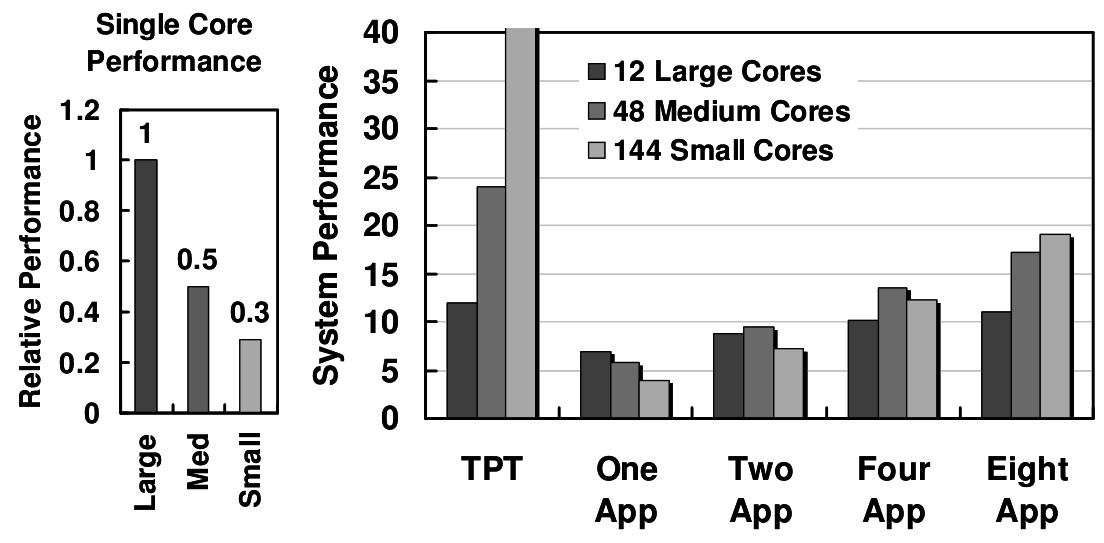
\includegraphics[height=0.4\textheight]{images/pollack.png}
            \\
            Amdahl's law &
            \pause
            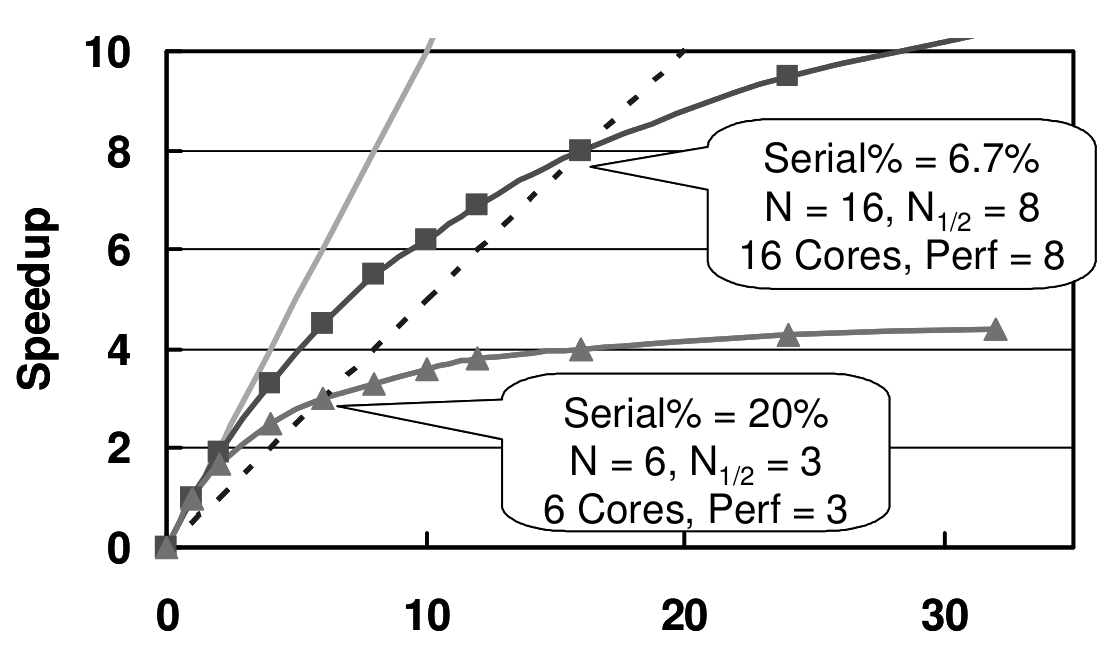
\includegraphics[height=0.4\textheight]{images/amdahl.png} \\
    \end{tabular}
\end{frame}

\begin{frame}{So?}
    \begin{itemize}
        \item Increase number of cores.
        \item And make them smaller.
            \pause
        \item \alert{Increase parallelism}
    \end{itemize}
    
\includegraphics[height=0.2\textheight]{images/orly.jpg}
\end{frame}

\end{document}
